\chapter{Introduction}

\section{The Hot Big Bang model}

The most accepted model for the origin of the universe is the Big Bang model, which surprisingly to some conveys no "bang", but the sudden existence of all the matter in the universe, in the shortest of times, in the smallest of spaces, about 13.8 billion years ago. After an unthinkably small interval of time, the universe began a short period of rapid expansion known as \textit{cosmic inflation}, in which the universe grew by a factor $10^{27}$ in a mere $10^{-33}$ seconds. This inflation is thought to be due to the inflaton, a quantum scalar field theory. It is theorized that it is the inflaton's vaccuum energy what caused the universe to expand as greatly.

As any quantum field\footnote{Quantum fields are a tool used by Quantum Field Theory (QFT) to more accurately describe particles and their interactions, at high enough energies} the inflaton presents fluctuations. This means, even in the vacuum state\footnote{To define vacuum in QFT is not as easy a task as it was in classical mechanics (or even non-relativistic quantum mechanics).These details go beyond the scope of this paper, and thus will not be dealt with} there is constant creation and annihilation of particles. These fluctuations are what cause anisotropies in the matter distribution of the universe, fact that will be important later in the article.

After the inflation phase, the universe cooled enough for what is known as the Quark-Gluon plasma to form. In this state, temperatures were high enough as to consider relativistic the random motion of the particles in it. After some cooling due to cosmic expansion, the combination between quarks to form hadrons was allowed, leading to what is known as the hadronic epoch. However, due to the short mean free path of the photons the universe is still opaque to electromagnetic radiation.

As the universe kept expanding the densities and the temperatures cooled, the existence of atoms was starting to be allowed, the $He^{+}$ and $H$ atoms. This period would finish at the universe age of $380,000$ years, moment known as recombination. Though the name `recombination' implies the fact that the universe used to be `combined' and then ceased to be so, it just comes from the fact that recombination was theorized before the Big Bang theory was thought of.

More precisely, recombination is thought of as the time in which Thomson Scattering stops being effective (the scattering cross section of this process becomes negligible and thus the photon mean free path grows considerably).

As soon as recombination ends, the excited electrons which are now orbiting neutral atoms, fall to a lower energy state, thus emmitting photons in great densities. This emmision is known as the Cosmic Microwave Background (CMB) and is the oldest direct measurement we can take of the unvierse.


\begin{figure}[h]
	\centering
	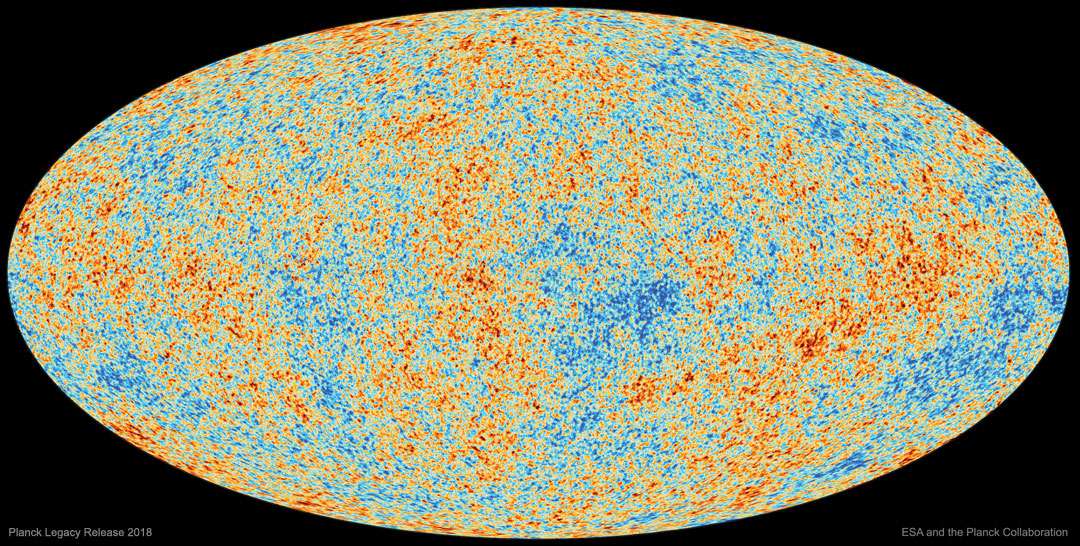
\includegraphics[width=0.8\textwidth]{../figs/cmb.jpeg}
\caption{The CMB as seen by Space-based Observatory Planck (cita collaboration 2018)}
	\label{fig:cmb}
\end{figure}
\section{Cosmic Microwave Background}

We see in the figure \ref{fig:cmb} the CMB as observed by the Planck colaboration (cita collaboration2018). The radiaton we observe is the photons that were emmitted about $13.8$ billion years ago. Since the CMB appears as a result of the thermal photons emitted by the electrons in the primordial plasma, it offers great insight into what the plasma looked like, and the way it behaved. 

The Cosmic Microwave Background was discovered in 1965 as a serendipity by Penzias and Wilson (cita penzias and wilson). They observed a noise signal, uniformly distributed\footnote{It was not actually uniformly distributed, since there was a small doppler shift due to the Earth's relative movement to the CMB. Surprisingly, even after removing this and other similar effects, it still presents minute fluctuations. These fluctuations, as it will be seen in the next sections contain a great deal of information on the structure of the universe.} from every direction, day or night, summer or winter. 	

Almost as if it came directly from the origin of the universe.

This discovery was considered to be solid evidence for the Big Bang model and more importantly, the beginning of the modern cosmology. All of this became the reason Penzias and Wilson received a Nobel prize 13 years later, in 1978.

Since what is being measured are the photons left from recombination, which corresponds to a thermal radiation curve, we may use Wien's law 
\begin{align}
	T = \frac{b}{\lambda}
\end{align}
with $b\approx $ \SI{2.897}{mmK} Wien's constant, $T$ the black body radiation and $\lambda$ the wavelength at which the spectral radiation is maximum to calculate the corresponding temperature to the measured wavelength. The measured wavelength is \SI{1.063}{mm} (microwave radiation, as the name implies) which corresponds to a temperature of \SI{2.72548}{K} with fluctuations of \SI{0.00057}{K}. 

These anisotropies were first measured by the COBE satellite in 1991 (cita SmootMather) and later earning Smoot and Mather a nobel prize. As of 2023 the most precise measurements correspond to the Planck experiment in 2018 (citar Planck2018) by the European Space Agency.

Of course, \SI{2.72548}{K} was not the temperature of the plasma at recombination, as it was approximately hotter by a factor $z=1090$, or $\approx$\SI{3000}{K}. The reason we measure such smaller temperatures is because of the expansion of the universe.

Thus, the CMB becomes crucial in explaining the large scale structure of the universe, since the photons that decoupled from the plasma at recombination wasted more energy leaving denser regions behind losing thermal energy in the process. 

\section{Baryon Acoustic Oscillations}

Before recombination, both matter and photons were coupled into the same fluid which we have called the primordial plasma. The particles in the plasma interacted primarily with one another through gravity and electromagnetism, depending on the type of matter considered. 

As already mentioned, matter was not distributed homogenously. At some point in time before recombination one could find `lumps' of dark and baryonic (standard) matter. Combining the restoring force of the gravitational attraction between dark and baryonic matter with itself and with one another, and the repulsion caused by the radiation pressure due to the Thomson Effect between baryons and photons, the results are pure acoustic waves propagating through the plasma, with the dark matter lumps being in the center of these waves. Since the waves propagated through baryonic matter, these waves are called Baryon Acoustic Oscillations (BAO).

The waves would propagate throughout the plasma as long as the baryon-photon interaction was strong enough i.e. up until recombination, at which point they froze in time leaving higher density regions. Higher density means higher gravitational intensity, which in turn means higher galaxy proliferation in spherical distributions. These spherical distributions (which can be measured in the CMB) are what is known as the large scale structure of the universe.

At big enough distances, the radii ($r_s$) of these spheres, also called the sound horizon is used as a `cosmic ruler'. Big scale measurements are calculated in terms of $r_s$, which is measured from the CMB, which means it needs to be calibrated from external information. $ r_s$ has been measured from the CMB to be around  \SI{150}{Mpc} or 500 million lightyears.

These structures were discovered in 2005 by D. Eisenstein (cita Eisenstein) and offer a great deal  of information about the size of the `cosmic ruler' of the universe, allowing better and better accuracy in big scale cosmic measurements. The radii ($r_s \approx 150 Mpc \approx 500 $ million lightyears) of the spherical waves, the sound horizon, can be measured both in the CMB radiation, as we have already seen, and through the nearby galaxies. It has been verified that the \textit{comoving} measurements\footnote{The distance measured if the cosmological expansion did not exist} of $r_s$ is constant throughout the universe.



\section{Curvature, dark matter and the expansion of the universe}
After Hubble discovered the expansion of the universe through Hubble's Law (cita articulo original hubble)
\begin{align}
	v = H_0 d
	\label{eq:ley-hubble}
\end{align}
With $v$ the recession speed (the speed at which some point in space is receeding only considering the expansion of the universe), $H_0=100h \frac{km}{s}Mpc ^{-1}$ Hubble's constant and $d$ the distance of said point, a great deal of studies concerning the expansion of the universe started. The most relevant result of those for this report are Friedmann's equations.
\begin{align}
	H^2(t) := \left(\frac{\dot a}{a}\right)^2 &=  \frac{8\pi G \rho}{3} +\frac{\Lambda c^2}{3} - K \frac{c^2}{a^2}
	\label{eq:1a-friedmann}\\
	3 \frac{\ddot a}{a} &= \Lambda c^2 - 4\pi G \left( \rho + \frac{3p}{c^2} \right) 
	\label{eq:2a-friedmann}
\end{align}
In these equations we see many new paramaters. $H(t)$ is a generalization of $H_0$, $H_0$ being the value of $H(t)$ at present time. $a(t)$ is the size factor of the universe, meaning that if a certain distance measurement $\Delta x$ was taken at time $t_1$, then that same measurement would be $\frac{a(t_2)}{a(t_1)}\Delta x$ at $t_2$. $G$ is the universal gravitational constant, $\rho$ the matter density of the universe (baryonic, dark matter, etc), $\Lambda$ is the cosmological constant which contains information about Dark Energy. Finally we see $K$, which is the Gaussian Curvature of the universe. This is, asymptotical curvature.

These equations are a result of the Friedmann–Lemaître–Robertson–Walker metric 
\begin{align}
	ds ^2 = -c^2 dt^2  + a^2(t) \left( \frac{dr^2}{1-kr^2} +r^2d\theta ^2 + r^2 \sin^2\theta d\phi^2\right) 
	\label{eq:FLRW}
\end{align}which are a direct result of solutions to Einstein's field equations of General Relativity, which will not be covered in this report. In \eqref{eq:FLRW} one sees the usual components in a flat space Minkowskian metric 
\begin{align}
	ds^2 = -c^2dt^2 + dr^2 + r^2d\theta^2 + r^2 \sin^2\theta d\phi^2
\end{align} and some new terms, $a(t)$ and $k$. $a(t)$ was the already mentioned scale factor, and $k$ a measure of the curvature of the universe. It is easier now to see that $a(t)$ is crucial in the way things are measured. Also, one can notice how having different types of universe affects differently to the metric. For example $k=0$ yields (as one would expect) a flat universe. $k>0$ corresponds to a universe with spherical geometry and $k<0$ to a universe of hyperbolical geometry.

If one managed to solve \eqref{eq:1a-friedmann}, the result would a description of the history of the expansion of the universe. Moreover, it is also important to notice the relationship between the expansion of the universe and the distribution of matter in the universe.

From \eqref{eq:1a-friedmann} we define the density parameter $\Omega_m$ as $\frac{\rho}{\rho_{\text{c}}}$, with the critical density $\rho_{\text{c}} = \frac{3H_0^2}{8\pi G}$, approximately the density of a cube of mass six times the mass of a proton and of volume \SI{1}{m^3}. Similarly from the rest of the terms in the equation \eqref{eq:1a-friedmann}
\begin{align}
 \Omega_\Lambda = \frac{\Lambda c^2}{3H^2}, \Omega_k = -K\frac{c^2}{H^2a^2} 
\end{align}
$\Omega_\Lambda$ corresponds to the density of dark energy in the universe, while $\Omega_k$ is not a density \textit{per se}, but is related to the energy of the universe due to its curvature.
These parameters are what define the certain cosmology we are using, and obey the cosmic sum rule 
\begin{align}
	1 = \Omega_m + \Omega_\Lambda + \Omega_k
\end{align}
Which is just a result of dividing \eqref{eq:1a-friedmann} by  $H_0^2$.

Historically, the concept of cosmological expansion appeared when Hubble observed that the radiation of the nearby galaxies was all shifted towards the red end of the spectrum. Of course, since the universe is expanding and the distance between two points increases with time, the wave length of a certain radiation would also be affected by this expansion. This stretching of the wave length is what is known as \textit{redshift} 
\begin{align}
	z = \frac{\lambda_{\text{o}} - \lambda_{\text{e}}}{\lambda_{\text{e}}} = \frac{\lambda_o}{\lambda_e} - 1
	\label{eq:redshift}
\end{align}
Being $\lambda_o$ the observed wavelength and $\lambda_e$ the emitted wavelength of the considered radiation. $z$ is a measure of how much the universe stretched while the radiation travelled, and it can be related to $a(t)$ through 
\begin{align}
	\frac{\lambda_o}{\lambda_e} = 1+z = \frac{a(t_o)}{a(t_e)}
\end{align}
Which means that $z$ is a temporal variable measuring the time the radiation travelled through the universe.

However, this redshift $z$ should not be confused with the redshift caused by the Doppler Effect of objects moving away. The processes are different in origin, since cosmological redshift does not need relative movement to shift the radiation towards red wavelengths, it is the expansion of the universe what stretches the wavelength. On the contrary, the Doppler Effect appears when pulses emmitted at regular time are emitted further away due to the movement of the wave source.

We thus define the comoving distance of a measurement $\Delta x$ as 
\begin{align}
	\frac{1}{1+z}\Delta x
\end{align}
i.e.\ the distance one would have measured had the expansion of the universe not existed.

With these definitions we can define  the observables we are interested in calculating/measuring. Firstly, through \eqref{eq:1a-friedmann} we calculate $H(z)$ as  
\begin{align}
	H(z) = H_0 \sqrt{\Omega_m(1+z)^3 + \Omega_k(1+z)^2 + \Omega_\Lambda} 
\end{align}
We also define the function of $z$ $D_H$
\begin{align}
	D_H(z)  = \frac{c}{H(z)}
\end{align}
Note that for $z = 0$ $D_H$ gives us an idea of the radius of the observable universe, i.e. the distance at which the recession speed is the speed of light in vacuum.

And the comoving line-of-sight distance as 
\begin{align}
	D_A = D_H\int_{0}^{z} \frac{dz}{\sqrt{\Omega_m(1+z)^3 + \Omega_k(1+z)^2 + \Omega_\Lambda} } 
\end{align}
